\section{mo\-Aspir\-Crit$<$ M $>$ Class Template Reference}
\label{classmo_aspir_crit}\index{moAspirCrit@{moAspirCrit}}
Description of the conditions in which a tabu move could be accepted.  


{\tt \#include $<$mo\-Aspir\-Crit.h$>$}

Inheritance diagram for mo\-Aspir\-Crit$<$ M $>$::\begin{figure}[H]
\begin{center}
\leavevmode
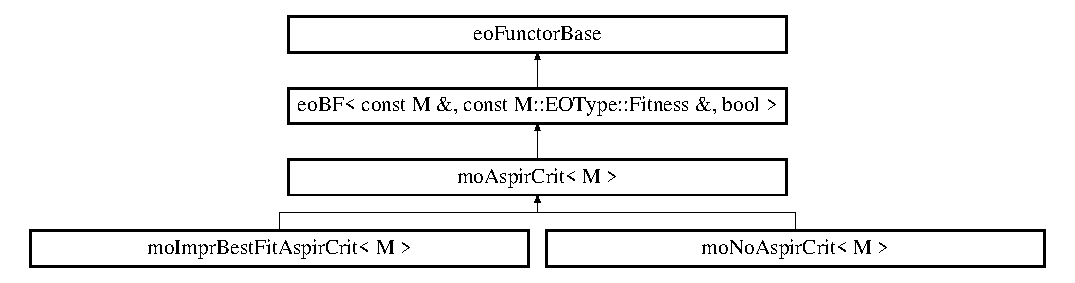
\includegraphics[height=3.35329cm]{classmo_aspir_crit}
\end{center}
\end{figure}
\subsection*{Public Member Functions}
\begin{CompactItemize}
\item 
virtual void {\bf init} ()=0
\begin{CompactList}\small\item\em Procedure which initialises all that needs an aspiration criterion. \item\end{CompactList}\end{CompactItemize}


\subsection{Detailed Description}
\subsubsection*{template$<$class M$>$ class mo\-Aspir\-Crit$<$ M $>$}

Description of the conditions in which a tabu move could be accepted. 

It is only a description... An object that herits from this class is needed to be used in a {\bf mo\-TS}{\rm (p.\,\pageref{classmo_t_s})}. See mo\-No\-Aspri\-Crit for example. 



Definition at line 47 of file mo\-Aspir\-Crit.h.

\subsection{Member Function Documentation}
\index{moAspirCrit@{mo\-Aspir\-Crit}!init@{init}}
\index{init@{init}!moAspirCrit@{mo\-Aspir\-Crit}}
\subsubsection{\setlength{\rightskip}{0pt plus 5cm}template$<$class M$>$ virtual void {\bf mo\-Aspir\-Crit}$<$ M $>$::init ()\hspace{0.3cm}{\tt  [pure virtual]}}\label{classmo_aspir_crit_a0}


Procedure which initialises all that needs an aspiration criterion. 

It can be possible that this procedure does nothing... 

Implemented in {\bf mo\-Impr\-Best\-Fit\-Aspir\-Crit$<$ M $>$} {\rm (p.\,\pageref{classmo_impr_best_fit_aspir_crit_a1})}, and {\bf mo\-No\-Aspir\-Crit$<$ M $>$} {\rm (p.\,\pageref{classmo_no_aspir_crit_a1})}.

The documentation for this class was generated from the following file:\begin{CompactItemize}
\item 
mo\-Aspir\-Crit.h\end{CompactItemize}
